\section{Concept}

In this chapter, we want to present the general concept of our approach by giving an overview of our architecture and explain the roles of each component. Afterwards, we will present the external data that is available for us and list all the requirements that we received from our external partner for the implementation of the interactive floorplan.

\subsection{System Overview}

To be able to meet the requirements of our interactive floorplan, the events from the gates need to be logged and displayed in real-time. For this to work, there are multiple components involved. A general overview of the architecture can be seen in figure ~\ref{fig:Komponentendiagramm}.

\begin{figure}[!hb]
    \centering
    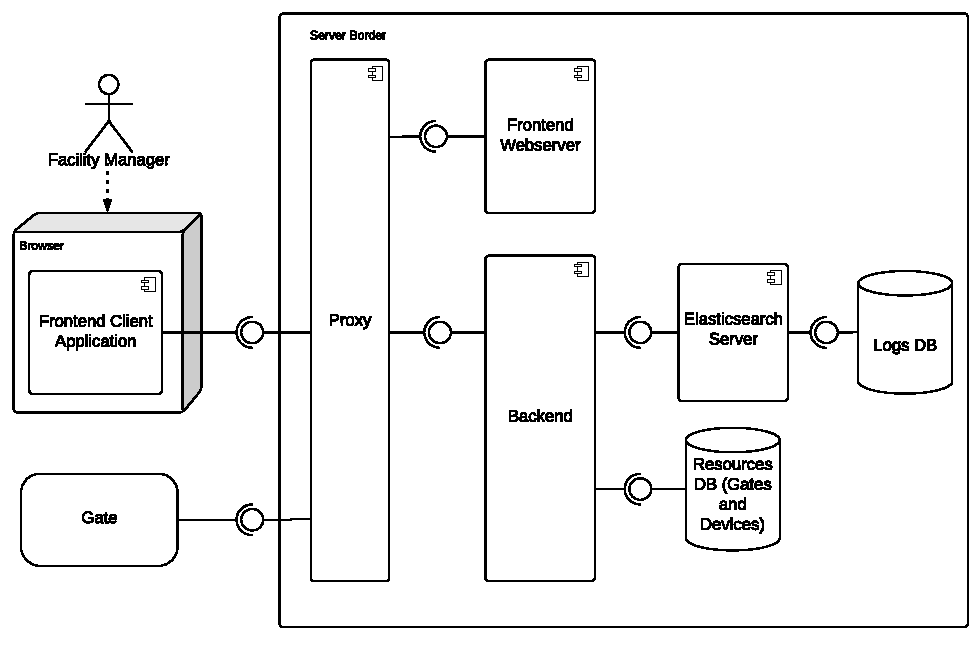
\includegraphics[width=1\linewidth]{images/Komponentendiagramm}
    \caption{Component diagram}
    \label{fig:Komponentendiagramm}
\end{figure}

\subsubsection{Gates}
\label{Gates}

The gates take care of capturing different pieces of information once a person tries to access through a gate. They gather information about the device that communicates with them, if they granted or denied access and if the person tries to enter or exit through the gate. In case of an alarm, they need to store other useful information about that incident.

The gate then is responsible for sending this information to our system via an API\footnote{Application Programming Interface}.


\subsubsection{Backend}
\label{Backend}

The backend offers interfaces for the gates and also the frontend. For the gates, it provides an interface that allows the gates to send events to, which then will be persisted as logs.
For the frontend, it provides routes for retrieving the logs and also analytical results based on these.

Once a gate transmits data through the available interface, the backend emits a notification that an event occurred together with the event data. 


\subsubsection{Frontend}
\label{Frontend}

The frontend presents the interactive floorplan to the facility management with clickable markers for each gate.
It features the adding and deleting of markers and the possibility to link them to a gate.
A click on a specific marker shows useful information about the gate, such as the minimum entry and minimum exit trust level required for this gate.

For the possibility of displaying data in real-time, it listens for the gate event notification sent from the backend. When a notification is emitted the frontend visualizes the event data to the user. This also triggers a recolorization of the room that is connected to the gate where the event occurred, thereby showing the up-to-date occupancy of that room.

\subsubsection{Logging Server}
\label{Logging Server}

The logging server takes care of storing the events in a log database. It offers endpoints for creating event logs and also for searching through the logs. This allows calculating the number of people in a room for example.

\subsection{External Input}

Multiple gates can be installed inside an office. We receive data about the access decisions made at these gates. We also get geospatial data for each indoor feature inside the office.

\subsection{Requirements}

\begin{itemize}
    \item \textbf{Interaction}:
    The floorplan should be an interactive map. This means that the user can interact with the map by zooming, panning of clicking, thereby altering the state and look of the map. This includes the possibility to set markers at a specific location on the map, which then can be linked with gates. A click on a marker then shows information about that specific gate.
    \item \textbf{Real-time Data Visualization}:
     The events from the gates should be displayed in real-time on the map. This includes information about the access, which enables to quickly view who entered at what gate at what time.
    \item \textbf{Eventlogging}:
    There needs to be an interface for the gates to send these events to. These need to be persisted as logs for later analytics.
    \item \textbf{Heatmap}:
    The plan should visualize the number of people in a room and render a "heat" on the map, thereby presenting the occupancy status of each room.
    \item \textbf{Alarm Localization}:
    The floorplan needs to visualize alarms, which is needed to locate threats on the map quickly.
    %\item \textbf{Upload Functionality}:
    %Because every user has different floorplans the upload of their own floorplans must be possible.
\end{itemize}

\clearpage



